\documentclass[tikz,border=8pt]{standalone}
\usepackage{amsmath,amssymb}
\usepackage{xcolor}
\usetikzlibrary{arrows.meta,positioning,fit,calc,backgrounds}
\definecolor{bg}{HTML}{071019}
\definecolor{panel}{HTML}{0C1520}
\definecolor{textc}{HTML}{F5F7FA}
\definecolor{muted}{HTML}{9DACBE}
\definecolor{gold}{HTML}{D0A94B}
\definecolor{orange}{HTML}{F18F6D}
\definecolor{violet}{HTML}{A88BFF}
\definecolor{cyan}{HTML}{62C7FF}
\definecolor{green}{HTML}{62D99B}
\definecolor{linec}{HTML}{40596F}
\begin{document}
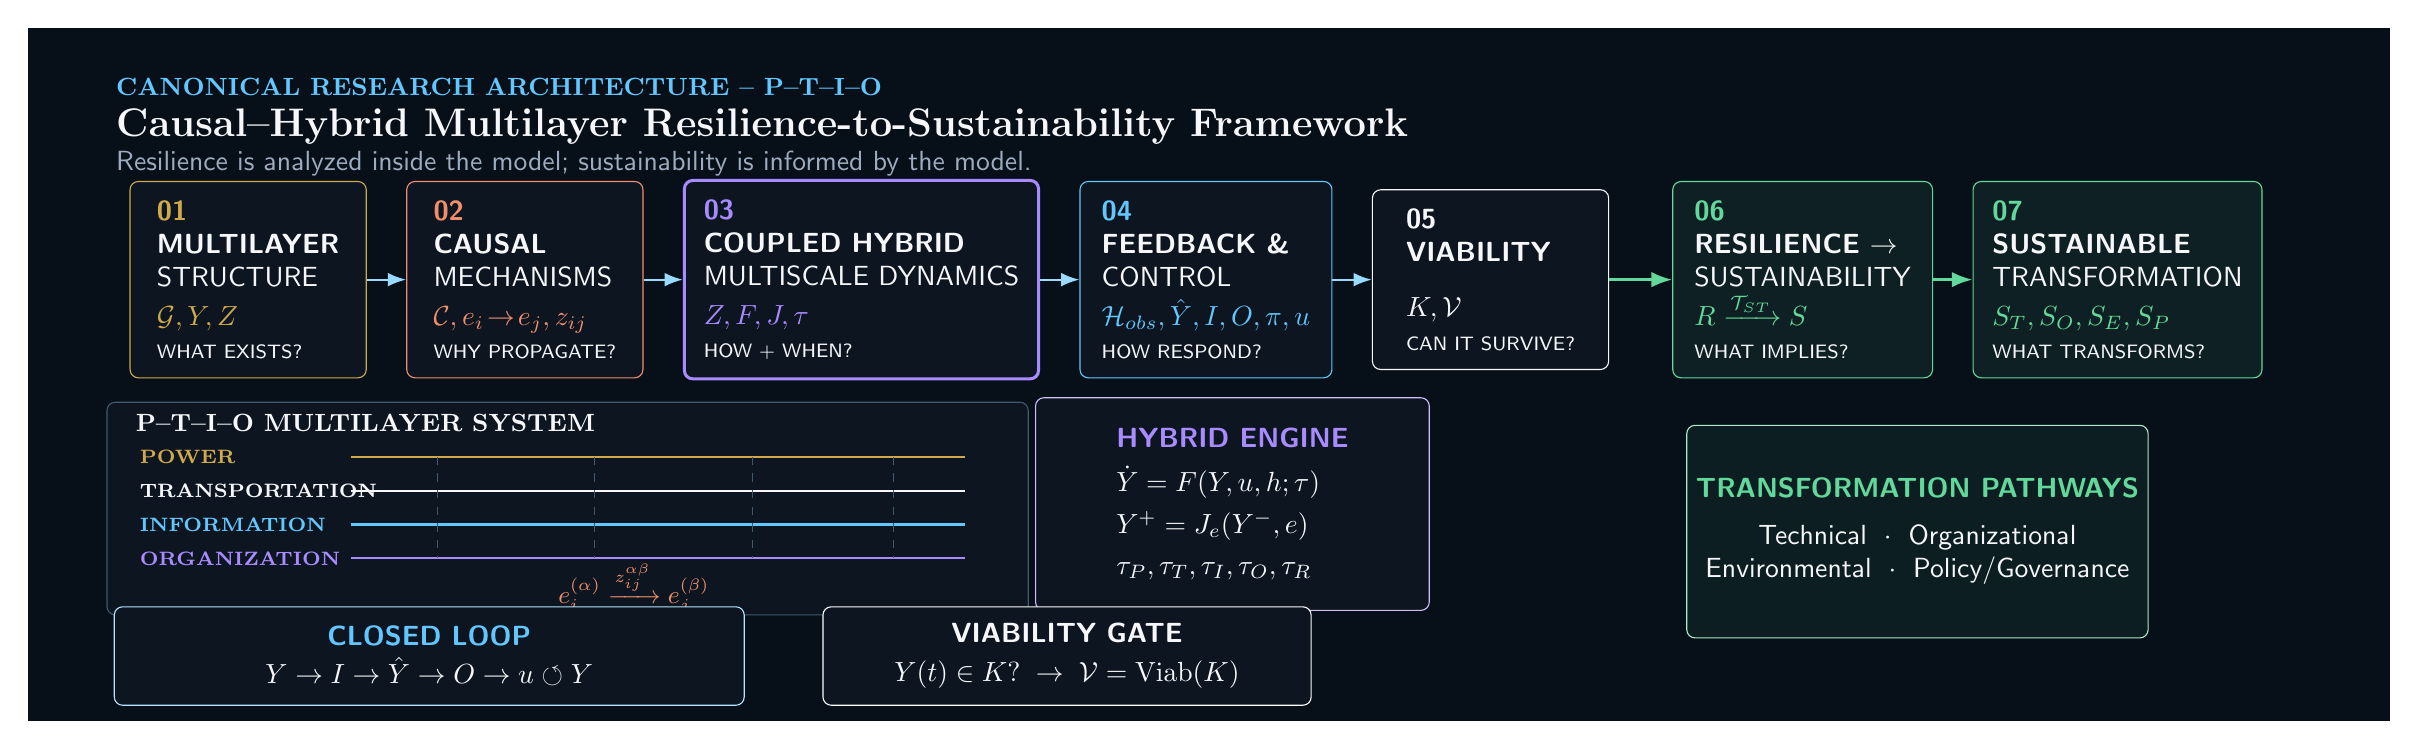
\begin{tikzpicture}[font=\sffamily, >=Latex, node distance=5mm and 5mm]
\fill[bg] (-1.0,-4.6) rectangle (29.0,4.2);
\node[anchor=west,text=cyan,font=\bfseries\small] at (0,3.45) {CANONICAL RESEARCH ARCHITECTURE -- P--T--I--O};
\node[anchor=west,text=textc,font=\bfseries\Large] at (0,2.95) {Causal--Hybrid Multilayer Resilience-to-Sustainability Framework};
\node[anchor=west,text=muted] at (0,2.48) {Resilience is analyzed inside the model; sustainability is informed by the model.};
\tikzset{stage/.style={draw=linec, fill=panel, rounded corners=3pt, minimum height=2.0cm, align=left, text=textc, inner sep=7pt}}
\node[stage,draw=gold,minimum width=3.0cm] (s1) at (1.8,1.0) {\textcolor{gold}{\bfseries 01}\\\bfseries MULTILAYER\\STRUCTURE\\[2pt]\textcolor{gold}{$\mathcal G,Y,Z$}\\{\scriptsize WHAT EXISTS?}};
\node[stage,draw=orange,minimum width=3.0cm,right=of s1] (s2) {\textcolor{orange}{\bfseries 02}\\\bfseries CAUSAL\\MECHANISMS\\[2pt]\textcolor{orange}{$\mathcal C,e_i\!\to\!e_j,z_{ij}$}\\{\scriptsize WHY PROPAGATE?}};
\node[stage,draw=violet,line width=1.1pt,minimum width=4.2cm,right=of s2] (s3) {\textcolor{violet}{\bfseries 03}\\\bfseries COUPLED HYBRID\\MULTISCALE DYNAMICS\\[2pt]\textcolor{violet}{$Z,F,J,\tau$}\\{\scriptsize HOW + WHEN?}};
\node[stage,draw=cyan,minimum width=3.2cm,right=of s3] (s4) {\textcolor{cyan}{\bfseries 04}\\\bfseries FEEDBACK \&\\CONTROL\\[2pt]\textcolor{cyan}{$\mathcal H_{obs},\hat Y,I,O,\pi,u$}\\{\scriptsize HOW RESPOND?}};
\node[stage,draw=textc,minimum width=3.0cm,right=of s4] (s5) {\textcolor{textc}{\bfseries 05}\\\bfseries VIABILITY\\[8pt]\textcolor{textc}{$K,\mathcal V$}\\{\scriptsize CAN IT SURVIVE?}};
\node[stage,draw=green,fill=green!8!bg,minimum width=3.3cm,right=8mm of s5] (s6) {\textcolor{green}{\bfseries 06}\\\bfseries RESILIENCE $\to$\\SUSTAINABILITY\\[2pt]\textcolor{green}{$R\xrightarrow{\mathcal T_{ST}}S$}\\{\scriptsize WHAT IMPLIES?}};
\node[stage,draw=green,fill=green!8!bg,minimum width=3.2cm,right=of s6] (s7) {\textcolor{green}{\bfseries 07}\\\bfseries SUSTAINABLE\\TRANSFORMATION\\[2pt]\textcolor{green}{$S_T,S_O,S_E,S_P$}\\{\scriptsize WHAT TRANSFORMS?}};
\foreach \a/\b in {s1/s2,s2/s3,s3/s4,s4/s5}{\draw[->,line width=.8pt,cyan!65] (\a.east)--(\b.west);}
\draw[->,line width=1pt,green] (s5.east)--(s6.west);
\draw[->,line width=1pt,green] (s6.east)--(s7.west);
\node[draw=linec,fill=panel,rounded corners=3pt,anchor=north west,minimum width=11.7cm,minimum height=2.7cm,text=textc,align=left] at (0,-0.55) {};
\node[anchor=west,text=textc,font=\bfseries\small] at (0.25,-0.82) {P--T--I--O MULTILAYER SYSTEM};
\foreach \yy/\lab/\col in {-1.25/POWER/gold,-1.68/TRANSPORTATION/textc,-2.11/INFORMATION/cyan,-2.54/ORGANIZATION/violet}{\node[anchor=west,text=\col,font=\bfseries\scriptsize] at (0.3,\yy) {\lab};\draw[\col,line width=.8pt] (3.1,\yy)--(10.9,\yy);}
\foreach \xx in {4.2,6.2,8.2,10.0}{\draw[dashed,linec] (\xx,-1.25)--(\xx,-2.54);}
\node[text=orange,font=\small] at (6.7,-3.0) {$e_i^{(\alpha)}\xrightarrow[\tau_{ij}]{z_{ij}^{\alpha\beta}}e_j^{(\beta)}$};
\node[draw=violet!55,fill=panel,rounded corners=3pt,minimum width=5.0cm,minimum height=2.7cm,text=textc,align=left] at (14.3,-1.85) {\textcolor{violet}{\bfseries HYBRID ENGINE}\\[4pt] $\dot Y=F(Y,u,h;\tau)$\\[3pt] $Y^+=J_e(Y^-,e)$\\[3pt] $\tau_P,\tau_T,\tau_I,\tau_O,\tau_R$};
\node[draw=cyan!45,fill=panel,rounded corners=3pt,minimum width=8.0cm,minimum height=1.25cm,text=textc,align=center] at (4.1,-3.78) {\textcolor{cyan}{\bfseries CLOSED LOOP}\\[2pt] $Y\to I\to\hat Y\to O\to u\circlearrowleft Y$};
\node[draw=textc!35,fill=panel,rounded corners=3pt,minimum width=6.2cm,minimum height=1.25cm,text=textc,align=center] at (12.2,-3.78) {\bfseries VIABILITY GATE\\[2pt] $Y(t)\in K?\;\to\;\mathcal V=\operatorname{Viab}(K)$};
\node[draw=green!55,fill=green!7!bg,rounded corners=3pt,minimum width=5.8cm,minimum height=2.7cm,text=textc,align=center] at (23.0,-2.2) {\textcolor{green}{\bfseries TRANSFORMATION PATHWAYS}\\[5pt] Technical $\;\cdot\;$ Organizational\\Environmental $\;\cdot\;$ Policy/Governance};
\begin{scope}[on background layer]
\node[draw=linec,rounded corners=4pt,fit=(s1)(s2)(s3)(s4)(s5),inner sep=5pt,label={[text=cyan,font=\bfseries\scriptsize]above:CORE RESILIENCE ANALYSIS}] {};
\node[draw=green!55,rounded corners=4pt,fit=(s6)(s7),inner sep=5pt,label={[text=green,font=\bfseries\scriptsize]above:SUSTAINABILITY EXTENSION}] {};
\end{scope}
\end{tikzpicture}
\end{document}
